\documentclass[12pt, a4paper, oneside]{ctexbook}
\usepackage{amsmath, amsthm, amssymb, bm, wallpaper}
\usepackage{graphicx, hyperref, mathrsfs, caption}
\usepackage{float, subfigure, enumerate, ulem, paralist}
\usepackage{cite, listings, color}
\usepackage[final]{pdfpages}

\CTEXsetup[format={\Large\bfseries}]{section}
\linespread{1.5}
\newtheorem{theorem}{定理}[section]
\newtheorem{definition}[theorem]{定义}
\newtheorem{lemma}[theorem]{引理}
\newtheorem{corollary}[theorem]{推论}
\newtheorem{example}[theorem]{例}
\newtheorem{proposition}[theorem]{命题}


\newcommand\bv[1]{\boldsymbol{#1}}
\newcommand\mb[1]{\mathbb{#1}}
\newcommand\mc[1]{\mathcal{#1}}

% \renewcommand{\qedsymbol}{}

\captionsetup{labelformat=default,labelsep=space} %去除冒号

\begin{document}

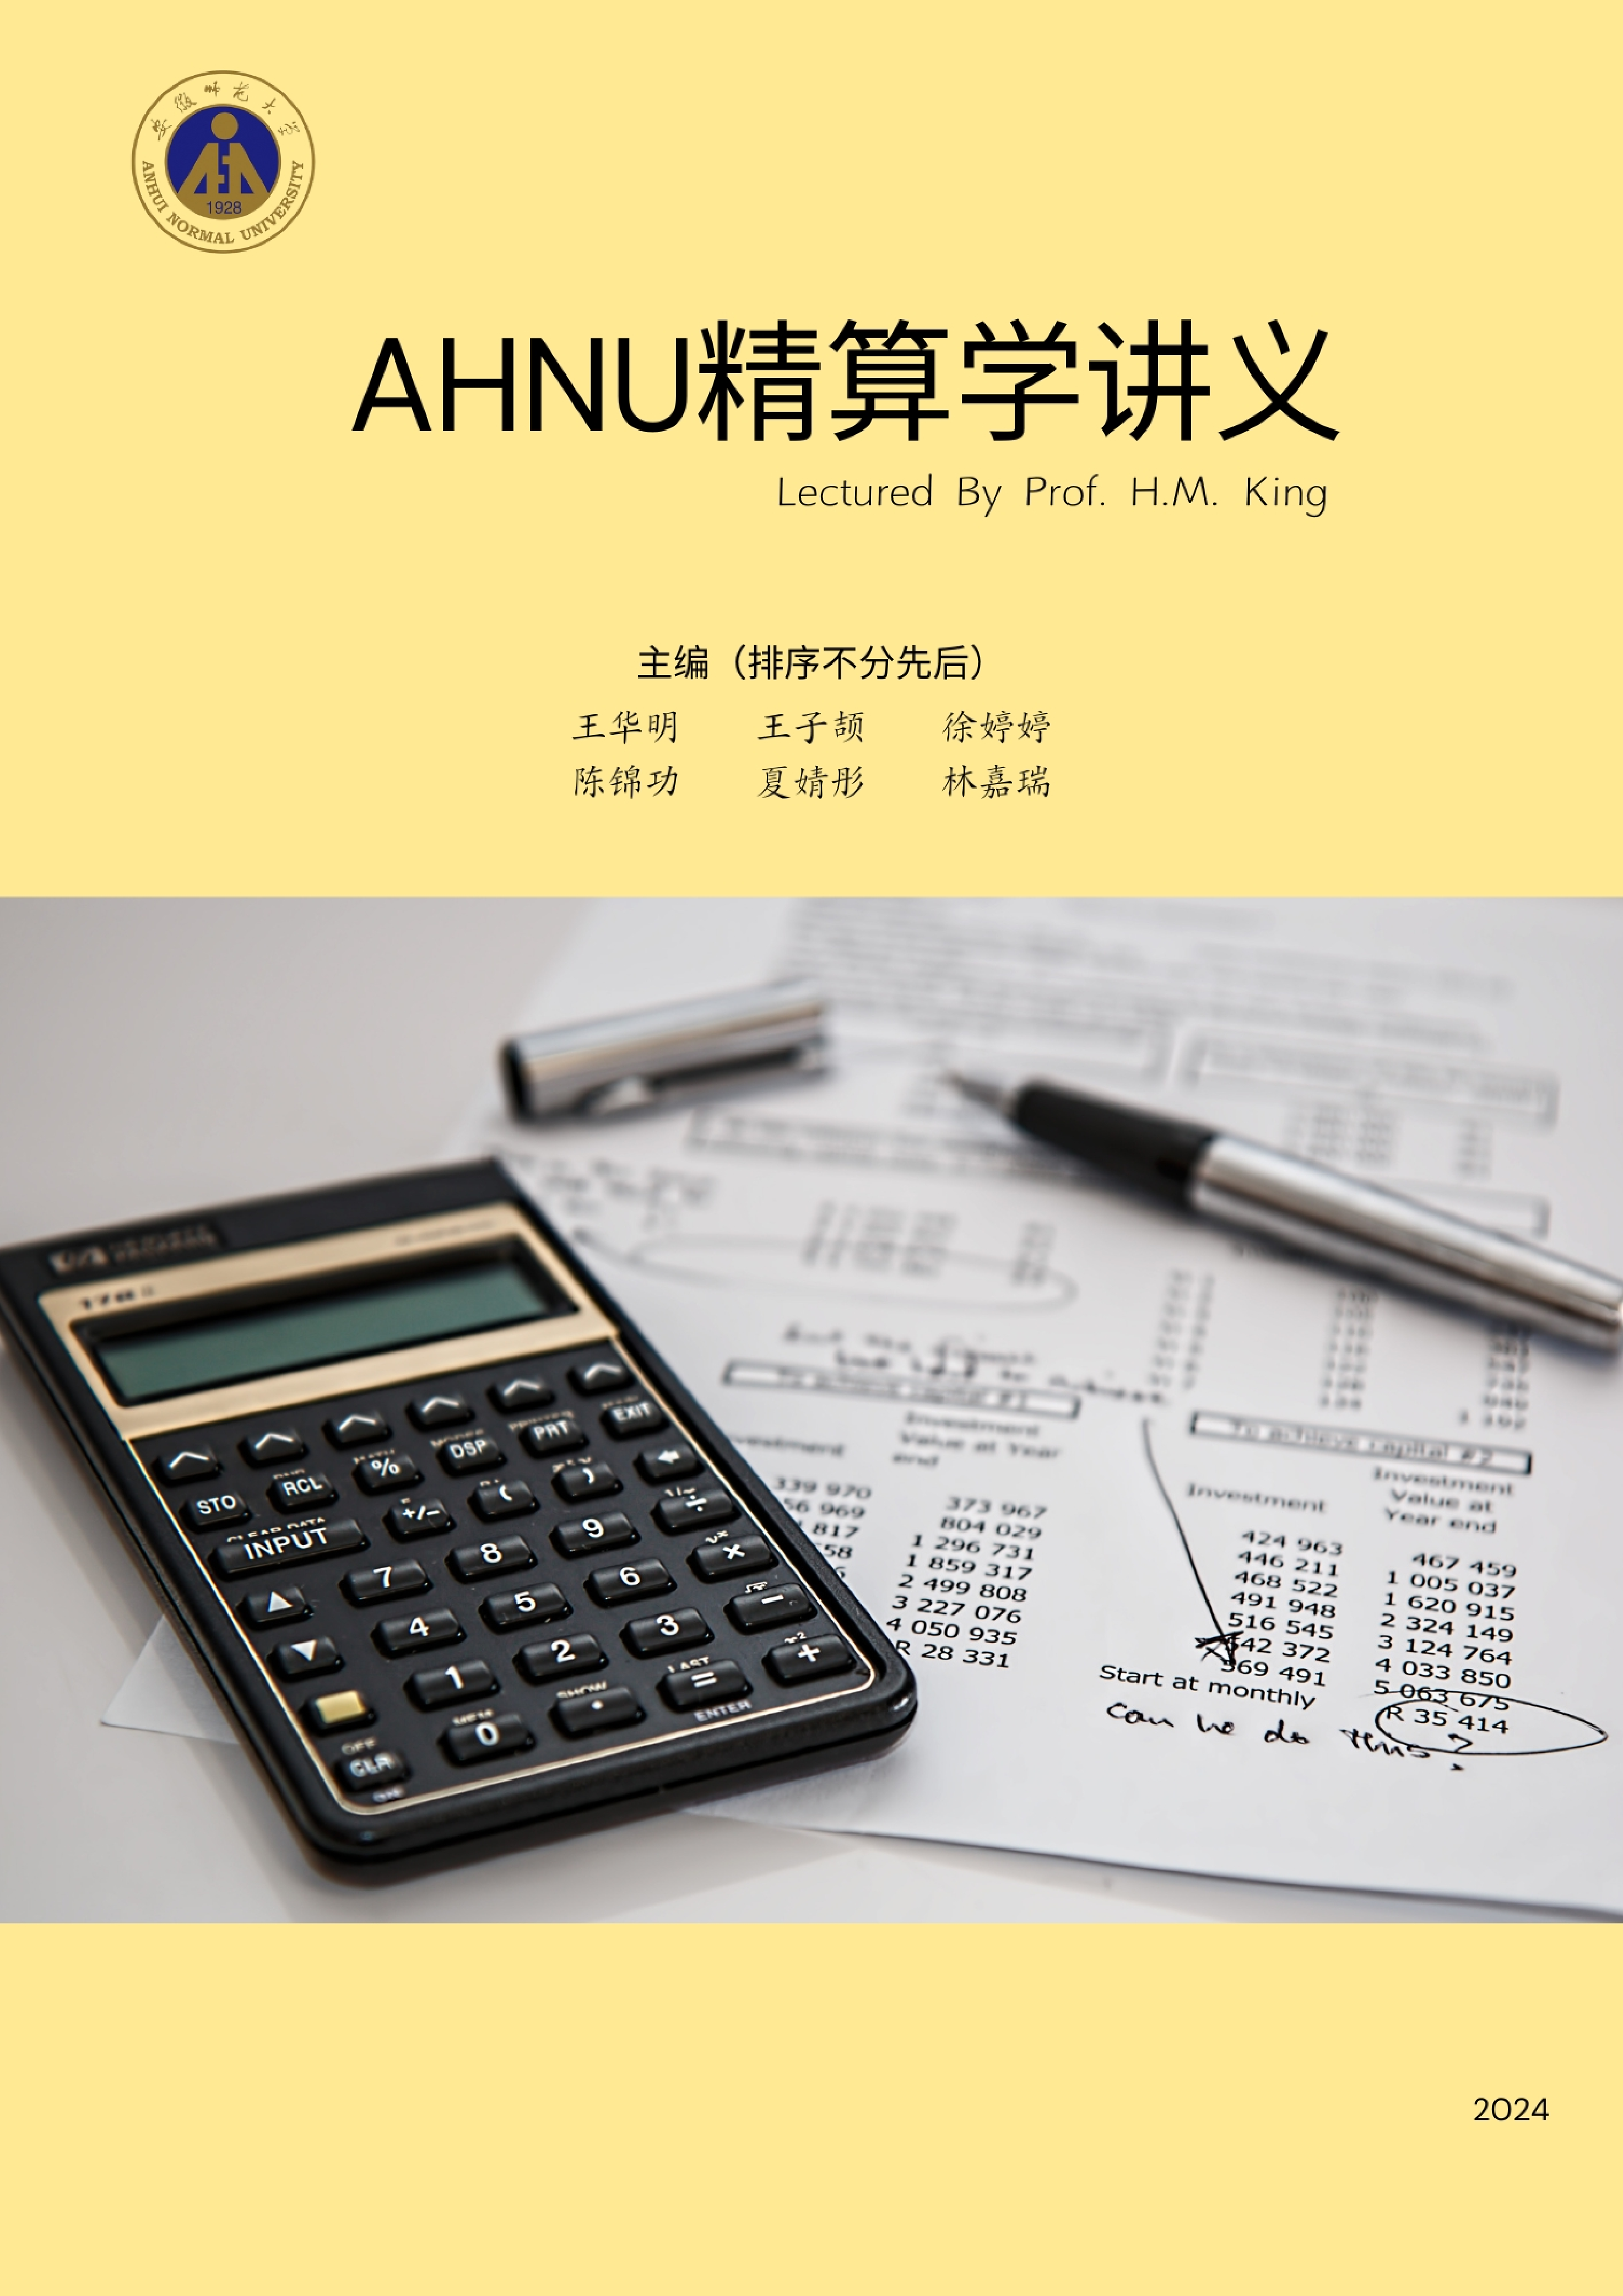
\includepdf{PDFCover.pdf}
\newpage
\title{{\Huge{\textbf{AHNU精算学讲义}}\\}}
\author{精算学讲义编写组}
\date{\today}



\pagenumbering{roman}
\setcounter{page}{1}



\begin{center}
    \Huge\textbf{前言}
\end{center}
\par 本讲义基于王华明老师在2023-2024年第二学期对安徽师范大学2021级统计学专业讲授的《精算学》课程。本讲义使用\LaTeX\ 编写,编者旨在整理课上课下相关内容。由于编者水平、时间有限,讲义中难免有谬误之处,欢迎各位发现错误和愿意提出改进建议的读者联系编者。

\newpage
\tableofcontents
\newpage
\pagenumbering{arabic}
\setcounter{page}{1}



\newpage
% \pagestyle{empty}
\section*{更新日志}
2024.2.28

由H.M. King老师领导的编写组成立,由WZJ和LJR完成了初步模板的编写。

\chapter*{精算学内容}
\begin{enumerate}[1、]
    \item 你能活多久?(生存分布)
    \item 你死的时候,保险公司支付你1元,这1元的现值为多少?(人寿保险)
    \item 在你活着时,保险公司给你1元,这些支付的现值是多少?(生存年金)
    \item 上述的寿险与生存年金,你该交多少保费?(保费理论)
    \item 为了保证支付,要准备多少钱?(准备金理论)
\end{enumerate}

\chapter{单生命生存模型}
\section{生存分布}
\subsection{新生儿的生存分布}
\textbf{1、生存函数:}设有一个新生儿,他的寿命记为$X$,$X$为一个非负的随机变量,以下总假设$X$为连续型随机变量。
\begin{definition}
    设$F_X(t)$是$X$的分布,$f_X(t)$是$X$的密度函数,$F_X(t) = \int_0^t f(s)\mathrm{d}s$,在$F_X(t)$的连续点上,有$f_X(t) = F_X'(t)$。称$s(t) = P(X > t) = 1 - F_X(t)$为$X$的生存函数。
\end{definition}

\textbf{2、死亡力:}
\begin{definition}
    某人在$t$时刻死亡的可能性大小,考虑极限
    \begin{equation*}
        \begin{aligned}
              & \lim_{\Delta t\to0+}\frac{P(t<X\leqslant t+\Delta t|X>t)}{\Delta t}         \\
            = & \lim_{\Delta t\to0+}\frac{P(t<X\leqslant t+\Delta t)}{\Delta tP(X>t)}       \\
            = & \lim_{\Delta t\to0+}\frac{F_X(t+\Delta t) - F_X(t)}{\Delta t}\frac{1}{s(t)} \\
            = & \frac{F_X'(t)}{s(t)} = \frac{f_X(t)}{s(t)}
        \end{aligned}
    \end{equation*}
    即$\frac{f_X(t)}{s(t)}$描述了某人在$t$附近死去的“速率”。称$\mu(t) = - \frac{s'(t)}{s(t)}$为新生儿在$t$处的死亡力函数。
\end{definition}

\begin{corollary}
    \begin{enumerate}[a.]
        \item $\mu(t) = -\frac{s'(t)}{s(t)} = \frac{f_X(t)}{s(t)} = \frac{f_X(t)}{1 - F_X(t)}$
        \item $f_X(t) = \mu(t)s(t) = \mu(t)e^{-\int_0^t \mu(s)\mathrm{d}s}$
        \item $s(t) = e^{-\int_0^t\mu(s)\mathrm{d}s}$
    \end{enumerate}
\end{corollary}

\begin{proof}
    $\mu(s) = -\frac{s'(s)}{s(s)} = -[\ln s(s)]'$
    , $\int_0^t\mu(s)\mathrm{d}s = -\ln s(t) + \ln s(0)$, 因$s(0) = P(X > 0) = 1$, 故$s(t) = e^{-\int_0^t\mu(s)\mathrm{d}s}$。
\end{proof}

\textbf{1、}$s(t) = e^{-\int_{0}^{t}\mu(s)\mathrm{d}s}, ~\mu(t) = -\frac{s'(t)}{s(t)}$,即生存函数$s(t)$与死亡力函数$\mu(t)$相互唯一确定。

\textbf{2、}一个函数$\mu(t)$要作为死亡力,必须满足以下两条:
\begin{enumerate}[(1).]
    \item $\mu(t) \geq 0, ~\forall t \geq 0$
    \item $\int_0^{\infty}\mu(t)\mathrm{d}t = \infty$
\end{enumerate}

\begin{example}
    设有一个新生儿的寿命$X \sim e(\lambda)$,$f_X(t) = \lambda e^{-\lambda t}, ~t \geq 0$,$F_X(t) = 1 - e^{-\lambda t}, ~t \geq 0$,$s(t) = 1- F_X(t) = e^{-\lambda t}, ~t \geq 0$。

    死亡力:$\mu(t) = -\frac{s'(t)}{s(t)} = \lambda, ~\forall t \geq 0$。

    由此可见,指数分布的死亡力是常数,表示新生儿在任意岁数死去的可能性一样大,即新生儿永远年轻,所以指数分布作为寿命分布是不合适的。
\end{example}

\textbf{3、整数年龄与分数年龄:}$X = K(0) + S(0)$,$K(0)$为整数部分,$S(0)$为分数部分。
记$\mathring{e}_0 = E(X)$,它表示新生儿的期望寿命,$e_0 = E(K(0))$表示期望整数寿命
\begin{equation*}
    e_0 \leq \mathring{e}_0 < e_0 + 1
\end{equation*}

\begin{lemma}\label{le1.1.5}
    设随机变量X的n阶矩存在,即$E(X^n) < \infty$,则$\lim_{t \rightarrow \infty}t^ns(t) = 0$
\end{lemma}
\begin{proof}
    \begin{equation*}
        \begin{aligned}
                 & t^n s(t) = t^nP(X>t)                                 \\
            =    & \int_{t}^{\infty} t^nf_X(s)\mathrm{d}s               \\
            \leq & \int_{t}^{\infty} s^nf_X(s)\mathrm{d}s \rightarrow 0
        \end{aligned}
    \end{equation*}
\end{proof}

\begin{corollary}
    \begin{enumerate}[a.]
        \item $\mathring{e}_0 = E(X) = \int_0^{\infty}s(t)\mathrm{d}t$
        \item $E(X^2) = \int_{0}^{\infty} 2ts(t)\mathrm{d}t$
        \item $E(K(0)^2) = \sum_{n = 1}^{\infty} (2n-1)s(n)$
        \item $E(K(0)) = \sum_{n = 1}^{\infty} s(n)$
    \end{enumerate}
\end{corollary}
\begin{proof}
    \begin{equation*}
        \begin{aligned}
            {E}\left(X^{n}\right) & =\int_0^\infty t^n\mathrm{d}F(t)=\lim_{M\to\infty}\int_0^Mt^n\mathrm{d}F(t)=-\lim_{M\to\infty}\int_0^Mt^n\mathrm{d}s(t) \\
                                  & \left.=-\lim_{M\to\infty}(\left[t^ns(t)\right]\right|_0^M-\int_0^Mnt^{n-1}s(t)\mathrm{d}t)                              \\
                                  & =\lim_{M\to\infty}[-M^ns(M)]+\lim_{M\to\infty}\int_0^Mnt^{n-1}s(t)\mathrm{d}t                                           \\
                                  & =\int_0^\infty nt^{n-1}s(t)\mathrm{d}t.
        \end{aligned}
    \end{equation*}
    a,b即证。
    \begin{equation*}
        \begin{aligned}
            E(K(0)^2) & = \sum_{K = 0}^{\infty} K^2P(K(0) = K)                            \\
                      & = \sum_{K = 0}^{\infty} K^2[P(X \geq K) - P(X \geq K+1)]          \\
                      & = \sum_{K = 0}^{\infty} K^2s(K) - \sum_{K = 0}^{\infty} K^2s(K+1) \\
                      & = \sum_{K = 0}^{\infty} (2K+1)s(K+1)                              \\
                      & = \sum_{n = 1}^{\infty} (2n-1)s(n)
        \end{aligned}
    \end{equation*}
    c即证。
    同理可证d。
\end{proof}

\subsection{X岁个体的生存分布}
一个$X$岁还活着的个体记为$(X)$,$(X)$的余命记为$T(X)$,$T(X)$的分布表示在已知$\{X\geq x\}$的条件下,$T(X) = X - x$。

记$F_{T(x)}$为$T(X)$的分布函数,则
$$
    \begin{aligned}
        F_{T(X)}(t) & = P(T(X) \leq t|X \geq x) = P(X- x \leq t | X \geq x) = \frac{P(X \leq t + x, X \geq x)}{P(X \geq x)} \\
                    & = \frac{P(X > x) - P(X > x + t)}{P(X > t)} = 1 - \frac{s(x+t)}{s(x)}
    \end{aligned}
$$

记$f_{T(X)}(t)$为$T(X)$的密度函数,则
\begin{equation*}
    f_{T(X)}(t) = F_{T(X)}'(t) = -\frac{s'(x+t)}{s(x)} = \frac{f_X(x+t)}{s(x)}
\end{equation*}

记$s_{T(X)}(t) = 1 - F_{T(X)}(t) = \frac{s(x+t)}{s(x)}$为$T(X)$的生存函数。

个体$(X)$的死亡力为
\begin{equation*}
    \begin{aligned}
          & \lim_{\Delta t\to0+}\frac{P(t<T(x)\leqslant t+\Delta t|T(x)>t)}{\Delta t}                      \\
        = & \lim_{\Delta t\to0+}\frac{P(t<T(x)\leqslant t+\Delta t)}{\Delta tP(T(x)>t)}                    \\
        = & \lim_{\Delta t\to0+}\frac{s_{T(x)}(t) - s_{T(X)}(t + \Delta t)}{\Delta t}\frac{1}{s_{T(x)}(t)} \\
        = & - \frac{s_{T(x)}'(t)}{s_{T(x)}(t)} = - \frac{\frac{s'(x+t)}{s(x)}}{\frac{s(x+t)}{s(x)}}        \\
        = & -\frac{s'(x+t)}{s(x+t)} = \mu(x+t)
    \end{aligned}
\end{equation*}
\begin{definition}
    称$\mu_x(t) = -\frac{s_{T(x)}'(t)}{s_{T(x)}(t)}$为$X$岁个体在$t$年后的死亡力函数。
\end{definition}

\begin{corollary}
    \begin{enumerate}[a.]
        \item $\mu_x(t) = \mu(x+t)$,表示x岁的个体在t年后的死亡力等于新生儿在x+t年后的死亡力。
        \item $f_{T(x)}(t) = s_{T(x)}\mu_x(t)$
        \item $s_{T(x)}(t) = e^{-\int_0^t\mu_x(s)\mathrm{d}s} = e^{-\int_0^t\mu(x+s)\mathrm{d}s} = e^{-\int_x^{x+t}\mu(s)\mathrm{d}s}$
    \end{enumerate}
\end{corollary}



\end{document}